\section{Methodology}
\label{sec:methodology}

To answer the research question this study uses a human-centered approach (often referred to as Design Thinking) commonly found in Human-Computer Interaction studies consisting of four phases; 1) user studies to \textit{understand} the user, 2) \textit{data collection} methods and analysis of the situation as field trials, 3) \textit{ideation} and experimental design of a prototype and 4) \textit{evaluation} and usability testing of the prototype \cite{jonathan_lazar_research_2017, zimmerman_research_2007}. This mixed-methods approach (both qualitative and quantitative)  helps understand occupants' needs and informs the design and technical set-up of the prototype evaluating the effectiveness by focusing on the user's needs from the start of the study \cite{rogers_moving_2017}. For the first phase, an online questionnaire was conducted to \textit{understand} occupants' awareness of indoor air quality (see Section \ref{sec:questionnaire}), for the second phase a lab setting was created with IAQ monitors to do \textit{data collection} and gain insight into environmental data which in turn informed phase three the \textit{ideation} and creation of the prototype. In the last phase participants \textit{evaluated} the prototype and performed usability tests.

\subsection{Case study building}

This study will be conducted in association with the Digital Interactions Lab \footnote{https://uva-dilab.com/} and will utilize the recently opened Lab42 \footnote{https://lab42.uva.nl/} building at the UvA Amsterdam Science Park \footnote{https://www.amsterdamsciencepark.nl/} as its primary case study location. Lab42 is an energy-neutral, flexible, and adaptable faculty building that facilitates collaborations among students, researchers, and businesses \cite{benthem_2022}. 

\subsubsection{Space usage}

The buildings's layout is strategically organized into different zones, each serving various functions, ranging from quiet individual work to spaces that allow for collaborative work. Lecture halls, learning rooms, and open learning spaces make up the two lower floors, with the upper four being primarily assigned to the university academic staff, meeting rooms, and external offices (see Appendix \ref{appendix:building}).The overarching interior theme in the design revolves around 'tech' and 'nature' aiming to cultivate a fresh, light, and warm comfortable ambiance. Lab42 is an example of a smart building or living lab where sensing devices are retrofitted throughout the building to automatically adjust lighting, temperature, and the focus of this research regulating air \cite{architects_lab42_2022}. This already provides a base of environmental data that can be used and extended for further analysis. Since most of the space within the building is designated as informal learning space and another large part of the building is designed as meeting rooms (see Appendix \ref{appendix:building}), working areas these functions of focussed work and collaborative meetings can be heavily influenced by reduced cognitive performance as a result of poor indoor air quality.

\subsection{Questionnaire survey}
\label{sec:questionnaire}

To understand and collect occupants' subjective awareness and satisfaction of IAQ  a survey was created to gather quantitative data within the building as a form of Post Occupancy Evaluation (POE) (see Appendix \ref{appendix:building}).


\subsubsection{Questions}
The questions were based on two POE studies with a focus on indoor air quality \cite{silva_post-occupancy_2017, son_perceived_2023} and used standardized questions (e.g. Q-bank) and scales (e.g. Likert-scale). The survey consisted of a total of 9 questions (5 multiple choice, 3 Likert scales, 1 not mandatory open question) consisting of questions about:

\begin{enumerate}
  \item \textit{Activity and occupancy:} the rough location the occupant is within the building, how often the occupants use the building for various activities, and how they would describe the occupancy in their current space.
  \item \textit{Awareness and satisfaction:} how aware the occupant is of the current air quality in the space, how the occupant perceives the air quality in the current space, and how satisfied the occupant is with the air quality in the current space.
  \item \textit{Health and cognitive symptoms :} if the occupant experiences any health or cognitive symptons based on the air quality in the current space.
\end{enumerate}


\subsubsection{Participants}
The survey was distributed via handouts with QR Codes using eligibility criteria based on demographic characteristics to occupants present at the informal learning spaces of the atrium, first floor, and second floor. There were no additional inclusion criteria besides the sample size of respondents being present in the case study building. Additionally, handouts were attached to the tables using stickers. All instances of participation were voluntary and conducted without remuneration. Distribution of the survey was open for participation for four weeks within the Lab42 building which recorded XX ($n$=XX) responses in total of which after cleanup a total of XX ($n$=XX) responses were included in the final dataset. On average, participants used the Lab42 building 3 times a week for various activities (min=1d, max=5d, Mdn=3d) and most occupants from the sample size were located on the ground floor (($f$=8)) as opposed to the first floor (($f$=34)) and 2th floor (($f$=34)). No personal identifiable information such as age and gender were collected during the survey and ethical considerations (e.g. consent forms) were taken into consideration (see Appendix \ref{appendix:building}).

\subsubsection{Data analysis}
\label{sec:analysis}
After the distribution of the survey completed analysis of the collected data was performed in the form of data cleanup and exploratory data visualization. In Python (Jupyter Notebook format) \footnote{https://jupyter.org/} Libraries such as Numpy \footnote{https://pandas.pydata.org/} were used to clean the data (e.g. remove non-consenting users) and visualization libraries such as Seaborn \footnote{https://seaborn.pydata.org/} were used to create graphs and plots (e.g. boxplot the likert-scales) to get an overview of the collected data and gain insight into understanding the occupants.

\begin{figure*}[!t]
    \centering
    \begin{subfigure}[b]{0.23\textwidth}
        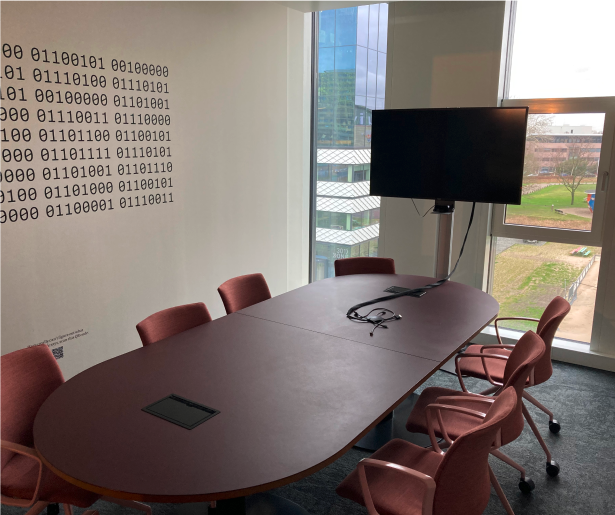
\includegraphics[width=\textwidth]{building.png}
        \caption{Figure 1}
        \label{fig:1}
    \end{subfigure}
    \hfill
    \begin{subfigure}[b]{0.23\textwidth}
        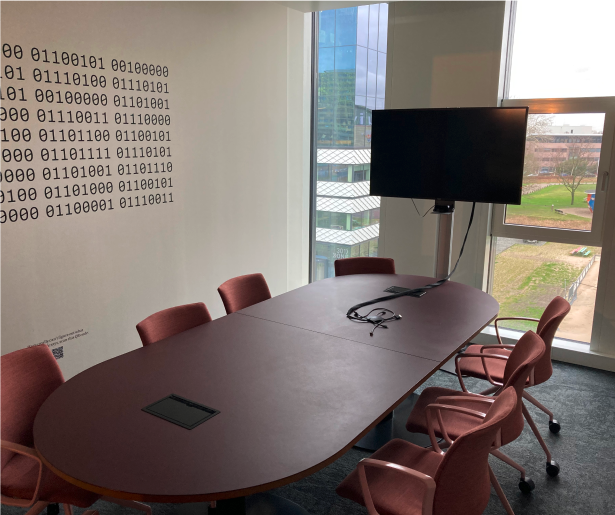
\includegraphics[width=\textwidth]{building.png}
        \caption{Figure 2}
        \label{fig:2}
    \end{subfigure}
    \hfill
    \begin{subfigure}[b]{0.5\textwidth}
        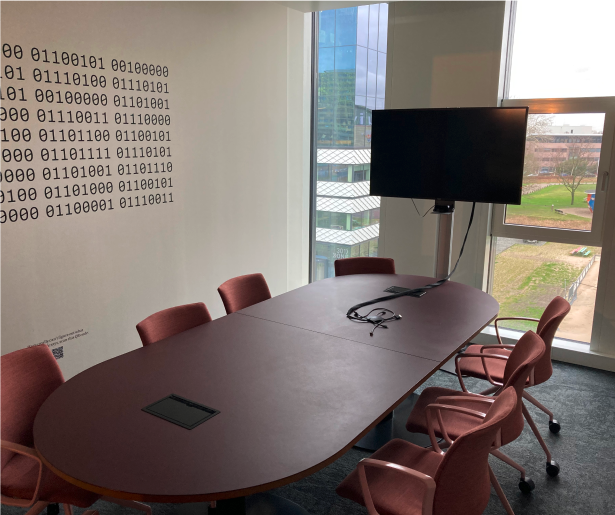
\includegraphics[width=\textwidth, height=0.38\textwidth]{building.png}
        \caption{Figures 3 and 4 combined}
        \label{fig:3_4_combined}
    \end{subfigure}
    \caption{Impressions of the ideations and prototyping phase}
    \label{fig:full_width}
\end{figure*}

\subsection{Air Quality Monitoring}

To gather data about the current situation of air quality within the building and understand the current situation within the building in terms of air quality data we retrofitted IAQ monitors (see Appendix \ref{appendix:building}) to two specific meeting rooms within the building.  This data collected was further used to inform and acts as a basis for the design of the data physicalisation (see \ref{sec:questionnaire} ).

\subsubsection{Technical set-up}

We deployed the monitors in meeting rooms occupants regularly use which allowed to understand occupants behavior and perception under real-world corporate settings as opposed to a controlled lab setting. We refer to them as the small room (room A) and the large room (room B). The small room’s is XX m2, and commonly used for small-size meetings (seven seats), while the large room’s ones is XX m2 (fourteen seats), which is more preferable for hosting larger-size meetings and seminars. Two commercially available indoor climate data loggers were installed using 3D printed mounting plates, a AirCheq Touch Aero \footnote{https://airteq.eu/producten/touch-aero/} in the smaller room and a Atal ATU-CT ClimaTrend \footnote{https://www.atal.nl/atu-ct-climatrend-binnenklimaat-datalogger} in the larger room. Both monitors use industry-standard (e.g. Senseirion and SenseAir) sensors to measure common pollutants and were mounted (e.g. between 80cm and 120cm from the ground) and calibrated (e.g. intervals, polling rates) as described by both manufacters installation manuals.

\begin{table}[htbp]
    \centering
    \caption{Sample Indoor Air Quality Data}
    \begin{tabular}{lccc}
        \toprule
        \textbf{Time} & \textbf{Humidity (\%)} & \textbf{VOCs (ppm)} & \textbf{CO2 (ppm)} \\
        \midrule
        08:00 & 40 & 0.05 & 500 \\
        09:00 & 42 & 0.06 & 520 \\
        10:00 & 45 & 0.07 & 550 \\
        \bottomrule
    \end{tabular}
    \label{tab:air-quality}
\end{table}

\subsubsection{Data logs}

The data gathered by the sensors provides insights into various standardized measurements related to common pollutants that affect IAQ such as molds and allergens (humidity), volatile organic compounds (VOC), and carbon dioxide (CO2) (see Table \ref{tab:air-quality}). We cross-referenced the data logs with two weekly schedules based on the internal booking systems of the rooms based on the timestamped data to align the values of the sensors from the data logs when meetings were scheduled.
Data analysis is performed similary as described in section \ref{sec:analysis} were data was cleaned to remove data from mainly non-opening hours and plotted and visualizated to visually explore patterns in the data and cross-reference them with meeting times.


\subsection{Ideation and requirements}

As a starting point for creating a physical representation of the air quality data we base our research on the growing interest in establishing theoretical and design foundations for \textit{data physicalisation} \cite{hornecker_design_2023, sauve_physecology_2022, bae_making_2022} on how to encode the properties and use a common design language \cite{ranasinghe_encoding_2023, sosa_data_2018} established by systematic reviews of data physicalization projects. The overall goal of the prototype is described in the following definition:

\AtBeginEnvironment{quote}{\setlength{\leftmargini}{10pt}}
\AtBeginEnvironment{quote}{\itshape}
\begin{quote}
a data-driven physical artifact whose geometry and material properties encode data that aims to augment a nearby audience’s understanding of data insights.
\end{quote}

Before prototyping the design solution we first describe the  intentions and scope of the physicalization. We derived five relevant dimensions based on the literature; \textit{audience, intention, interaction, philosophy, representation} \cite{sauve_physecology_2022, hornecker_design_2023}.

\subsubsection{Design philosophy}

Minimize interuption cost, notion of calm technology, ideal situation use persuasive techniques to help them take preventive actions.

\subsubsection{Data representation}

Write about data scale (stevens) nominal, ordinal and numerical. Needs electronic components (e.g. microcontrollers, sensors) and non-electronic components.

\subsubsection{Audience}

\subsubsection{Intention}

\subsubsection{Interaction}

\subsubsection{User requirements}

Based on this scope and the survey we describe the user requirements ("UR" for "User Requirements") of the design solution in further detail in the form of requirements, in user story format, ranked based on the MoSCoW method:

\begin{enumerate}
    \renewcommand{\labelenumi}{UR\arabic{enumi}:}
    \item The system should provide a user-friendly interface.
    \item Users should be able to register for an account with a valid email address.
    \item Upon registration, users should receive a confirmation email.
    \item The system should allow users to log in securely using their credentials.
    \item Users should be able to create, update, and delete their profiles.
\end{enumerate}

\subsubsection{Concept models}

For the concept models two existing datasets were used as a starting point for brainstorming and inspiration. First was the DataPhys gallery \footnote{http://dataphys.org/list/gallery/}, a collection of 372 entries classified as data physicalizations. The second was a combination of three state of the art papers with systematic reviews of physicalization with a combined examples of around 132 entries classified as data physicalization of which both academic and non-academic samples. Out of these twelve ($f$=12) entries (($f$=8) academic, ($f$=4)) were selected for further review based on the similitary and aligment with the  before described dimensions of which three ($f$=3) projects (Physikit, other, other)with a focus on the environmental property of air (but not necessarily air quality within indoor environments). Additionally 

\subsubsection{Concept diagrams}

Based on the user requirements and ideation and concepting from the Communication and Multimedia Design (CMD) Methods Pack \footnote{https://cmdmethods.nl/} and Design Method Toolkit \footnote{https://toolkits.dss.cloud/design/} by the Digital Society School (DSS) three low fidelity (lo-fi) concepts were further elaborated (see Figure \ref{fig:complexity}) in order to choose one to create for the user studies and evaluation. 


\begin{enumerate}
  \item \textbf{Concept-1: Desk Planter (Aspen)}
      A desk planter or tree in the corner of the room with soil in it.Follows the organic growth of a 'seed' of a flower or tree from seed to sprouts to full flower. The better the air quality the more or faster the plant grows. Movement of the leaves can indicate the wind.

  \item \textbf{Concept-2: Hanging Sculpture (Bluebird)}
      A hanging planter type set-up with strings that 'grow' from the ceiling. Fresh air makes movement of the strings. People can walk by, feel the material (e.g. humidity). Can touch, allows most interactivity. Taking inspiration from kinetic sculptures and hanging / floating sculptures.

  \item \textbf{Concept-3: Wall Kinetic (Crocus)}
      A moss-like structure on the wall with flower bulbs embedded. The flowers 'open up' based on better fresh air. Taking inspiration from kinetic sculptures.
\end{enumerate}


Concept selection was based on weighted physicalization criteria from the literature, a harris profile  and expert reviews ($N$=4) feedback. Also technical limitations of the provided hardware (e.g. real-time data output of monitors, cost of hardware, availability of electronic components,) and limitations in the technical set-up of the building (e.g. space in the meeting rooms, not allowed to alter furniture) were choosing criteria. Based on aggregration of these criteria the \textit{Bluebird} concept was chosen to be further developed into a high-fidelity prototype.


\subsection{Prototype}

Based on the requirements, data physcalization desgin principles and concept models exploration a final high fidelity (hi-fi) version of the prototype was developed that functioned as a proof-of-concept of the physical design solution and utilised in the user study for evaluation.



\subsubsection{Concept description}

\textit{Bluebird} (see Figure \ref{fig:complexity}) is a hanging kinetic type sculpture inspired by organic nature materials and the shapes of hanging planters that encode the environmental properties of indoor air quality data. It is meant to be hang from the ceiling in small to medium rooms (xM2) and changes based on real-time air quality monitor data. Strings (plant branches) either become lengtheir or smaller simulating the growth of a plant. Movements of the leaves indicate the freshness of air and movement.

\subsubsection{Electronics and components}

A controller device running on a Arduino Uno R3 \footnote{https://store.arduino.cc/products/arduino-uno-rev3} microcontroller with a MKR Motor shield is used \footnote{https://store.arduino.cc/products/arduino-motor-shield-rev3} to control six 360° MG90S type Micro Servo Motors \footnote{https://www.towerpro.com.tw/product/mg90s-3/}. Attached to these motors are pulleys with fishing line simulating the growth of the hanging planter and so that the string can be moved up and down.


\subsubsection{Crafting technologies and materials}
The strings, leaves and housings of the electronics and mechanical hardware are created using additive manufacturing (3D Printing) using a Fused deposition Modeling (FDM) technique using Polylactic acid (PLA) plastic filament in various colors. The electronics enclosures and plant models were modeled using computer-aided design (CAD) software. A digital fabrication technique commonly found in data physcalization prototypes \cite{anhalt_university_germany_design_2022}. To create leaves representing textile or fabric custom properties were defined withing the 3D printing software (Slicing) to remove top and bottom layers and create a thin layer of infill.

\subsubsection{System Architecture and software}

The microcontroller uses custom firmware written in Arduino code \footnote{https://www.arduino.cc/reference/en/} (similar to C++) that receives real-time data from the air quality monitors using the LoRaWAN \footnote{https://lora-alliance.org/about-lorawan/} communication protocol to control the mechanics of the prototype. This arrangement of hardware is commonly found in Internet of Things (IoT) architecture set-ups and follows the notion of Edge Computing with a (1) sensing, (2) networking, (3) processing and (4) application layer \cite{li_edge-oriented_2019, idrees_edge_2018}.

\begin{figure}[!h]
    \centering
    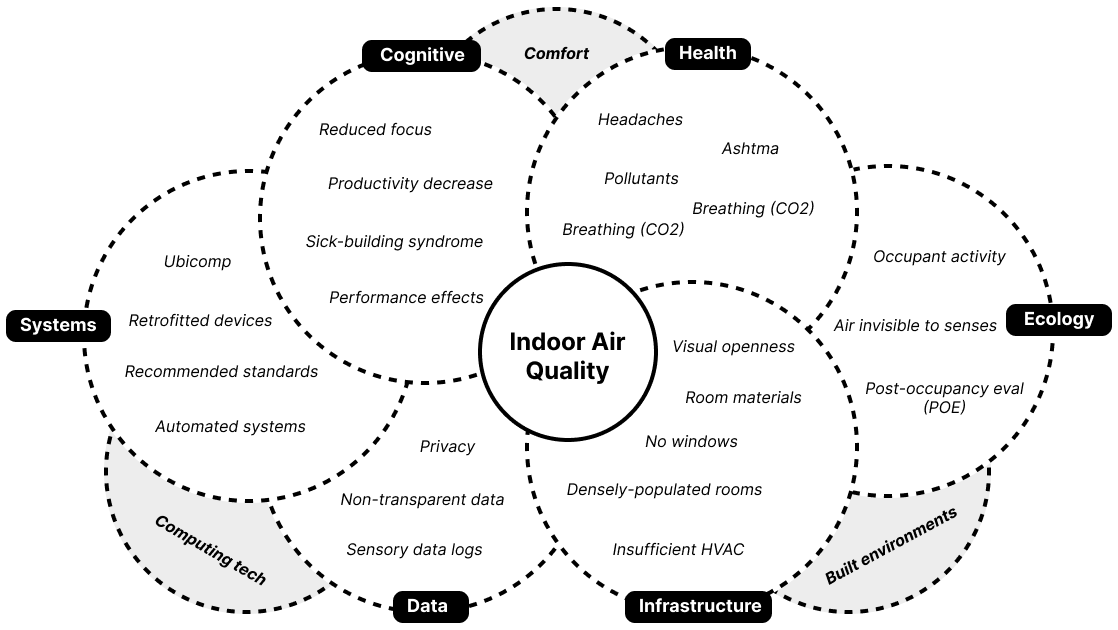
\includegraphics[width=0.5\textwidth]{complexity_diagram_indoor_air_quality.png}
    \caption{Complexity diagram providing an overview of the effects of IAQ and needs of occupants \cite{schweizer_indoor_2007, wang_how_2021, kim_analyzing_2019, alavi_comfort_2017, corlan_importance_2021, klepeis_national_2001}}
    \label{fig:complexity}
\end{figure}

\subsection{Evaluation}

The prototype was evaluated using common performance-related criteria that are widely used in HCI/Information Visualisation \cite{ranasinghe_encoding_2023} and Grounded Theory studies \cite{chun_tie_grounded_2019}. We employed a field-based evaluation approach with accompanying methods (see Section \ref{sec:questionnaire}) based on the Human-centered Design Kit by Ideo \footnote{https://www.designkit.org/methods.html} and Delft Design Guide from the Delft University of Technology (TU) \footnote{https://www.bispublishers.com/delft-design-guide-revised.html}. For evaluation criteria we used the intentions described in \cite{ranasinghe_encoding_2023} and interview methodology similar to \cite{jansen_evaluating_2013} as a baseline for evaluating the efficiency, memorability in in-person evaluation sessions. To measure the overall effectiveness and usability of the physicalization we used an adoptation of the Technology Acceptance Model (TAM) to gather insight into perceived usefulness, attitutde towards using and system usability scale \cite{}. 

\subsubsection{Hypothesis elicitation}

On the basis of the research question and creation of the prototype four hypothesis ("H" for "Hypothesis") were formulated to evaluate on.

\begin{enumerate}
    \renewcommand{\labelenumi}{H\arabic{enumi}:}
    \item The system should provide a user-friendly interface.
    \item Users should be able to register for an account with a valid email address.
    \item Upon registration, users should receive a confirmation email.
    \item The system should allow users to log in securely using their credentials.
    \item Users should be able to create, update, and delete their profiles.
\end{enumerate}

\subsubsection{Participant sampling}

The sample size of evaluation interviews was 8 ($n$=8) and accepted because the study findings reached saturation, meaning that new interviews did not yield new insights after the first five interviews. Participants were gathered through purposive sampling, as respondents had to meet the inclusion criteria ("C" for "Criteria") that needed to be checked before the interviews: 

\begin{enumerate}
    \renewcommand{\labelenumi}{C\arabic{enumi}:}
    \item The participant needed to use a meeting room with the building a minimum of once a week
    \item The participant needed to work within the case study week a minimum of 3 days per week
\end{enumerate}

This resulted in a sample of X male, X female, consisting of various roles; from researchers from different labs, PhD candidates working at the labs to private company employees encompassing a range of ages (min=X, max=X, Mdn=X, IQR=X) and education levels. Participants used the meetings rooms on average X (min=X, max=X, Mdn=X, IQR=X) a week and worked within the lab42 building X (min=X, max=X, Mdn=X, IQR=X) a week.

\subsubsection{Semi-structured interviews}

Within the meeting-room lab set-up in the presence of the developed prototyped pre-arranged, semi-structured individual qualitative interviews were conducted with open-ended and nonleading questions (see Appendix \ref{appendix:building}). The goal was to gather first impressions and gain insight into how occupants understand the communicated data factors of the prototype.

\subsubsection{Participant observation}

After the explorative questions participants were encouraged to in more detail view the prototype and interact with it as a field trial stating anything they noticed. Participants behavior was observed within the meeting rooms and participants were encouraged to think aloud when viewing and interacting with the prototype (see Appendix \ref{appendix:building}). Informal leading questions were asked about improvements, design optimizalization and visual changes. The goal was to test the usability of the prototype and gather insight into the self-reflective properties of the prototype. 

\subsubsection{Effectiveness of the prototype}

After the interviews and observations, the participants were asked to fill in a digital online with structured pre-defined questions form rating several properties of the prototype for their effectiveness (see Appendix \ref{appendix:building}). The goal was to gather quantitative measurements about the usability and effectiveness of the prototype.

\subsubsection{Transcription and coding}
All interviews were anonomyzed and conducted in-person on-site and audio recorded with permission of the participants. The recordings were then verbatim transcribed using the build-in Microsoft 365 transcription tool \footnote{https://www.microsoft.com/nl-nl/microsoft-365} to avoid bias while note-taking. The transcribed interviews as textual data was processed via Atlas.ti \footnote{https://atlasti.com/} for qualitative coding.